\documentclass[12pt]{article}
\usepackage[papersize={8cm,12cm},margin={.5cm,.5cm}]{geometry}
\usepackage{common}
\begin{document}
\begin{problem}
  \item[6.] 圖(二)中有一個邊長 $5$ 公分的正方體。若此正方體的體積為 $V$ 立方公分,且表面積為 $A$ 平方公分,則下列敘述何者正確?
  \begin{figure}[ht]
    \centering
    \vspace*{-1ex}
    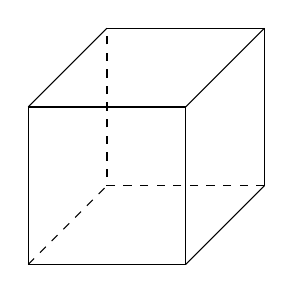
\begin{tikzpicture}
      \draw (0,0) -- (0,2) -- (2,2) -- (2,0) -- (0,0);
      \draw (1,3) -- (3,3) -- (3,1);
      \draw[dashed] (3,1) -- (1,1) -- (1,3);
      \draw[dashed] (0,0) -- (1,1);
      \draw (0,2) -- (1,3);
      \draw (2,2) -- (3,3);
      \draw (2,0) -- (3,1);
    \end{tikzpicture}
    \vspace*{-1ex}
    \caption*{圖(二)}
    \vspace*{-2ex}
  \end{figure}
  \begin{choices}
    \item $V = 100$
    \item $V = 200$
    \item $A = 50$
    \item $A = 150$
  \end{choices}
\end{problem}
\end{document}
